\documentclass[fontsize=12pt,paper=a4,toc=listof,bibliography=toc,headings=small]{scrbook}

% Quellcode
\usepackage{minted}
\usemintedstyle{perldoc}
\setminted{
  linenos,
  numbersep=4pt,
  autogobble,
  frame=lines,
  framesep=4mm
}
% Kompatibilität mit scrbook
\usepackage{scrhack}

% deutsche Umlaute
% \usepackage{lmodern}
\usepackage[T1]{fontenc}
\usepackage[utf8]{inputenc}
\usepackage{textcomp}

% deutsche Silbentrennung
\usepackage[english,ngerman]{babel}
\usepackage[autostyle]{csquotes}

% Bilder
\usepackage{graphicx}
\graphicspath{{../Kapitel/Grafiken/}}

% exakte Platzierung von Grafiken
\usepackage{float}

% Tabellen
\usepackage{booktabs}
\usepackage[table]{xcolor}
\usepackage{tabularx}
\newcolumntype{Y}{>{\centering\arraybackslash}X}
\newcolumntype{s}{>{\hsize=.3\hsize}X}
\usepackage{multirow}
% mit mehreren Zeilen
% \usepackage{array}

% Setzen der Seitenabstände
\usepackage{geometry}
\geometry{a4paper, top=30mm, left=40mm, right=20mm, bottom=30mm,
headsep=12.5mm, footskip=12.5mm}

% kleinerer Abstand vor Kapitelüberschrift
\RedeclareSectionCommand[
  beforeskip=24pt
]{chapter}

% leeres Endblatt
\usepackage{afterpage}
\newcommand\blankpage{
  \null{}
  \thispagestyle{empty}
  \addtocounter{page}{-1}
  \newpage
}

% biblatex
\usepackage[
  style=ieee,
  sorting=nyt,
  backend=biber]{biblatex}
\addbibresource{sources.bib}
\DefineBibliographyStrings{ngerman}{
  urlseen = {Abruf am}
}

% automatische Verlinkung
\usepackage{hyperref}
\hypersetup{
    colorlinks,
    citecolor=black,
    filecolor=black,
    linkcolor=black,
    urlcolor=black
}

% Layoutboxen anzeigen
% \usepackage{showframe}

\newcommand{\zB}{z.~B.\@}

\title{Abschlussarbeit}
\date{\today}
\author{Fabian Meyertöns}

\begin{document}
\frontmatter
\thispagestyle{empty}
\begin{center}
\Large{Hochschule für Technik und Wirtschaft Dresden}\\
\end{center}


\begin{center}
\Large{Fachbereich Informatik/Mathematik}
\end{center}
\begin{verbatim}





\end{verbatim}
\begin{center}
\textbf{\LARGE{Bachelorarbeit}}
\end{center}
\begin{verbatim}


\end{verbatim}
\begin{center}
\textbf{im Studiengang Wirtschaftsinformatik}
\end{center}
\begin{verbatim}
















\end{verbatim}

\begin{flushleft}
\begin{tabular}{lll}
\textbf{Thema:} & & Vergleich der Web API Ansätze REST und GraphQL\\
% & & Thema Zeile 2\\
& & \\
& & \\
& & \\
\textbf{eingereicht von:} & & Fabian Meyertöns\\
& & \\
& & \\
\textbf{eingereicht am:} & & \today \\
& & \\
& & \\
\textbf{Betreuer:} & & Prof.\ Dr.-Ing. Thomas Wiedemann
\end{tabular}
\end{flushleft}

\cleardoubleoddpage{}
\pagenumbering{Roman}
\tableofcontents \listoffigures \listoftables
\cleardoubleoddpage{}
\pagenumbering{arabic}

\mainmatter{}
\chapter{Einleitung}

\section{Motivation und Zielstellung}
\begin{itemize}
  \item Entwicklung von Web Anwendungen über die Zeit vom Monolith zu Service-orientierter Architektur
  \item Entwicklung vom Thin-Client zum Fat-Client, vom Server zu Services.
  \item Single Page Applikationen gesamte Kommunikation über Web APIs
  \item Vielzahl von internen Services im Unternehmen und externen Serviceanbietern führt zu wachsender Komplexität
  \item Einheitliche Kommunikation zwischen Client und Services ist wichtig.
  \item REST hat sich etabliert als Architekturkonzept, bleibt aber Implementierungsdetails schuldig. Verschiedene Standards und Dateiformate versuchen Einheitlichkeit zu schaffen und Komplexität zu verringern.
  \item GraphQL, 15 Jahre nach REST veröffentlicht, schafft festes Regelwerk/Protokoll für Client-Server Kommunikation, erfordert aber Umdenken und sehr verschiedene Implementierung.
  \item Frage für bestehende Anwendungen und APIs nach Migration zu GraphQL\@.
  \item Ersetzt GraphQL REST\@? Bei welchen Anwendungszwecken kann es als Ersatz dienen, bei welchen nicht?
  \item Welche neuen Probleme entstehen erst durch GraphQL\@?
  \item Ist ein gemeinsamer Einsatz von REST und GraphQL sinnvoll und möglich?
\end{itemize}
\section{Aufbau der Arbeit}
\begin{itemize}
  \item Betrachtung der Entwicklung von Web Anwendungen mit der Client-Server Architektur als Grundlage
  \item Abgrenzung des Begriffes API und Differenzierung von anderen API Ansätzen
  \item Das REST Architekturkonzept als Grundlage für das Web und APIs
  \item GraphQL als Alternative, seine Funktionsweise
  \item Vergleich von REST und GraphQL
  \item Welchen klassischen Problemen müssen sich API Entwickler stellen?
  \item Welche Probleme von REST löst GraphQL\@?
  \item Welche Vorteile hat REST gegenüber GraphQL\@?
  \item Vorstellung einer Auswahl von Tools und Bibliotheken, die verschiedene Probleme von REST und GraphQL lösen bzw.\ die Entwicklung vereinfachen.
  \item Untersuchung der Kompatibilität von Bibliotheken
  \item Tests von REST und GraphQL in verschiedenen Szenarien.
  \item Kombinierter Einsatz von GraphQL und REST
\end{itemize}
\chapter{Vorbetrachtungen}
\section{Client-Server Architektur}
\begin{itemize}
  \item Client-Server ist ein verteiltes System
  \item Zwischen Client und Server geschieht Nachrichtenaustausch
  \item Client fordert eine Operation vom Server an. Server sendet Resultat der Operation an den Client zurück.
  \item Client initiiert die Interaktion. Server reagiert.
  \item Mehrere Clients können den gleichen Server nutzen. Abbildung aus `Grundkurs verteilte Systeme'!
  \item Client kann mehrere Server benutzen. Server kann in anderer Interaktion selbst zum Client/Vermittler werden.
  \item Vorteile
    \begin{itemize}
      \item getrennte Entwicklung
      \item unabhängige Ausfälle
      \item Festgelegte Rollenverteilung: Client ist Konsument. Server ist Produzent.
    \end{itemize}
  \item Herausforderung: einheitliches Kommunikationsprotokoll
\end{itemize}
Die Basis für die meisten Anwendungen im Web bildet die Client-Server Architektur.
Der Nachrichtenaustausch in einem verteilten System wird dabei auf zwei Akteure und eine Interaktion fokussiert.
Der Client initiiert die Interaktion, indem er eine Nachricht an den Server sendet.
Der Server reagiert, indem er mit dem Resultat der Auswertung der Nachricht antwortet.
Ein Client kann mit mehreren Servern in Interaktion treten und mehrere Clients können mit dem gleichen Server kommunizieren.
Durch die Anfrage werden die Rollen von Client und Server festgelegt, welche jedoch nur für die Dauer der Interaktion gelten.
So kann ein Akteur, der bei einem Nachrichtenaustausch als Server angefragt wird, während eines anderen selbst als Client die Kommunikation beginnen.
Bedingung für die Client-Server Architektur ist, dass dem Client zu Beginn der Kommunikation, der Server bekannt ist und dass beide das gleiche Kommunikationsprotokoll unterstützen.
\par
Die Entwicklung einer Anwendung nach dieser Architektur hat ein erklärtes Ziel und Hauptvorteil: Die Trennung der Verantwortlichkeiten.\cite[vgl.][]{REST}
\par
Client und Server sind logisch und oft auch physikalisch getrennte Teile einer Anwendung und können unabhängig voneinander entwickelt werden, solange sie ihre Kommunikationsschnittstelle wahren.
Die damit verbundene Trennung der Verantwortlichkeiten führt zu einer Reduzierung der Komplexität der einzelnen Anwendungen.
Da Client und Server unabhängig voneinander ausgeführt werden, beeinflusst der Ausfall des einen nicht die Stabilität des anderen.
Wird der Client als Benutzeroberfläche und der Server als Datenspeicher genutzt, so können beispielsweise mehrere Clients für verschiedene Geräte oder Anwendungsfälle entwickelt und optimiert werden, wodurch die Portabilität der Oberfläche verbessert wird.
Die Verteilung auf mehrere Geräte erhöht außerdem die Skalierbarkeit des Gesamtsystems.

\section{Web APIs}
\begin{itemize}
  \item API bezeichnet Application Programming Interface
  \item Grundsatz ist die Kommunikation zweier Programme zur Konsumierung von anderem Quellcode, Abstraktion und Verstecken von Implementierungsdetails und Komplexität.
  \item Frameworks und Bibliotheken vieler Programmiersprachen bieten oft benötigte Funktionalität. Kommunikation besteht aus Aufruf mit Parametern und Antwort mit Ergebnis.
  \item Die Arbeit beschäftigt sich nur mit API von verteilten Systemen.
  \item Hauptaugenmerk auf Systemen mit Fat-Client. Großer Teil der Anwendungslogik auf Clientseite. Server dient als Datenspeicher. Hauptinteraktionen mit CRUD (Create, Read, Update, Delete)
  \item Popularität von Cloudservices und öffentlichen APIs bzw. Interaktion mit externen Services
\end{itemize}

\section{Abgrenzung zu anderen Web API Ansätzen}
\begin{itemize}
  \item SOAP (Simple Object Access Protocol), XML basiert, nutzt nur POST
  \item RPC (Remote Procedure Call), Zentraler Punkt ist das Aufrufen von Anwendungslogik auf dem Server, nicht Datentransport.
\end{itemize}

\chapter{Das REST Architekturkonzept}
\section{Entstehung}
Das Architekturkonzept des Representational State Transfer wurde erstmals im Jahr 2000 von Roy T. Fielding erwähnt, definiert und mit dem Akronym REST bezeichnet.\cite[76]{REST}
Es enthält eine Reihe von Prinzipien für die Entwicklung von verteilten Systemen im Web mit besonderem Fokus auf den Schnittstellen zwischen den einzelnen Komponenten.
Dabei baut REST auf der Client-Server-Architektur auf und hatte durch die Arbeit vib Fielding in den HTTP- und URI-Arbeitsgruppen direkten Einfluss auf die Entwicklung von der beiden Standards, wodurch jene Schnittstellen im Web definiert werden.\cite[vgl.][4,105f.]{REST}
REST beschreibt größtenteils die Architektur des Web selbst und ist daher nicht auf APIs ausgelegt oder beschränkt.

\section{Grundlagen}
\subsubsection{Ziele von REST}
Die Ziele und Vorteile der REST Architektur lassen sich folgendermaßen zusammenfassen:
\foreignblockcquote{english}[105]{REST}{REST provides a set of architectural constraints that, when applied as a whole, emphasizes scalability of component interactions, generality of interfaces, independent deployment of components, and intermediary components to reduce interaction latency, enforce security, and encapsulate  legacy  systems.}
Diese Ziele werden erreicht durch eine Reihe von Anforderungen.
\subsubsection{Komponenten und Prinzipien}
Die REST Architektur baut auf der weit verbreiteten Client-Server Architektur auf und definiert den Begriff der Ressource als Abstraktion für jede Art von Information, die Ziel einer Client-Anfrage ist.\cite[vgl.][88f.]{REST}
Als Beispiele für Ressourcen nennt Fielding selbst: \textcquote[88]{REST}{a document or image, a temporal service [\dots], a collection of other resources, a non-virtual object (e.g.\ a person).}
Eine Ressource wird durch einen Bezeichner bekannt gemacht und ist damit für einen Client abrufbar.
Der Bezeichner bleibt gleich, selbst wenn sich die damit identifizierte Ressource ändert.
Die Kommunikation einer Ressource vom Server zum Client erfolgt über eine Repräsentation der Ressource, d.h.\ ein Datenformat, welches vom Server festgelegt, oder durch Content-Negotiation zwischen Client und Server ausgehandelt wird.
Somit bleibt der Ursprung der Daten hinter der Serverschnittstelle versteckt.
Die Antwort des Servers enthält die Daten der Repräsentation und deren Metadaten.
Anfrage und Antwort enthalten außerdem Kontrolldaten, \zB{} HTTP Request Methods, Status Codes und Header, um die Bedeutung der Nachricht zu vermitteln.\cite[vgl.][90f.]{REST}
\begin{table}[h!]
  \begin{center}
    \caption{REST Data Elements}\label{tab:REST Data Elemens}
    \begin{tabularx}{\textwidth}{XXX}
      \toprule
      \textbf{Data Element} & \textbf{Web Equivalent} & \textbf{Example}\\
      \midrule
      resource & the intended conceptual target of a hypertext reference & a list of events\\
      resource identifier & URI & http://example.com/events\\
      representation data & HTML, JSON Document, PNG image & \{events:[\{title:\dots\},\{\dots\}]\}\\
      representation metadata & media type, last-modified time, ETag & Content-Type: application/json\\
      & & Content-Encoding: gzip\\
      control data & if-modified-since, cache-control, request method & GET, Cache-Control: no-cache\\
    \end{tabularx}
  \end{center}
\end{table}
\par
REST ist zustandslos, sodass jede Anfrage vom Client zum Server alle für deren Verarbeitung notwendigen Informationen beinhalten muss.
Ein Client speichert gewöhnlich seinen Zustand, während auf Serverseite keine Zustandsinformationen über mehrere Anfragen hinweg gespeichert werden, wie es zum Beispiel bei Sessions der Fall ist.
Aufgrund dieser Eigenschaft wird im Zusammenhang mit REST auch von einer \foreigntextcquote{english}[83]{REST}{Client-Cache-Stateless-Server[-Architektur]} gesprochen.
Hieraus ergeben sich drei Vorteile:\cite[vgl.][79]{REST}
\begin{itemize}
  \item Sichtbarkeit:
  Jede Anfrage kann separat untersucht und gecacht werden, ohne weitere Informationen zu benötigen.
  \item Zuverlässigkeit:
  Anfragen können atomar betrachtet und bei Teilfehlern kann ein stabiler Systemzustand leicht wiederhergestellt werden.
  \item Skalierbarkeit:
  Da ein Server Zustandsinformationen nur für die Dauer der Verarbeitung einer Anfrage speichert, können Ressourcen schnell wieder freigegeben werden.
\end{itemize}
Nachteil dieser Anforderung ist eine verringerte Netzwerkperformance, da bei sequenziellen Anfragen an einen Server, Daten zur Clientidentifikation, Authentifizierung oder aus vorangegangene Antworten erneut gesendet werden müssen.
Die verringerte Kopplung führt ebenfalls dazu, dass die Kontrolle des Servers über das Verhalten der Clientanwendung reduziert wird.
\par
Clientseitiges Speichern von erhaltenen Daten (Caching) erlaubt die Wiederverwendung früherer Serverantworten für zukünftige, gleiche Anfragen und ist sinnvoll, da die gefühlte Performance durch Verringerung der durchschnittlichen Latenz erhöht wird.
Dadurch wird die Effizienz und Skalierbarkeit der Anwendung erhöht, obwohl die Latenz jeder einzelnen Anfrage durch den Cache-Lookup erhöht wird.
Je mehr die gespeicherten Daten von den tatsächlichen Daten abweichen, desto mehr verringert sich die Verlässlichkeit derselben.\cite[vgl.][80]{REST}
GET-Requests werden von Webbrowsern implizit gecacht, wobei Server das gewünschte Caching-Verhalten explizit erlauben und verbieten können.

REST beschreibt drei Typen von Komponenten:\cite[vgl.][96]{REST}
\begin{itemize}
  \item User Agent:
  Dies kann ein Webbrowser bzw.\ die Benutzeranwendung sein, in jedem Fall jedoch der letztendliche Empfänger der Antwort.
  \item Origin Server:
  Die endgültige Quelle der Repräsentation einer Ressource und der letztendliche Empfänger von Request, die zu Modifikationen der Daten führen.
  \item Intermediary (Zwischenkomponenten):
  Diese befinden sich zwischen User Agent und Origin Server und können sowohl als Client, als auch als Server agieren. Sie leiten Anfragen und Antworten weiter, können diese aber auch modifizieren. Je nach Anwendungsfall spricht man hier von einem Gateway oder Proxy.
\end{itemize}
Für die Schnittstellen der Komponenten gelten folgende Grundsätze:\cite[vgl.][82]{REST}
\begin{itemize}
  \item Ressourcen müssen durch einen Bezeichner eindeutig identifizierbar sein.
  \item Die Interaktion mit einer Ressource, d.h.\ das Abfragen und Manipulieren derselben erfolgt über eine Repräsentation der Ressource.
  \item Nachrichten müssen so selbsterklärend sein, dass sie von der Schnittstelle verstanden und verarbeitet werden können.
  \item \foreigntextcquote{english}[82]{REST}{hypermedia as the engine of application state} (HATEOAS): Der Hypertext beschreibt den Zustand der Anwendung und die Möglichkeiten der Veränderung desselben.
\end{itemize}
\par
Durch die generischen Client- und Serverschnittstellen, die selbstbeschreibenden Nachrichten und die zustandslose Kommunikation kann eine REST Anwendung leicht von Schichten profitieren.
Keine einzelne Komponente benötigt Kenntnis des gesamten Informationsweges, sondern sieht nur die Komponenten, mit denen sie direkt interagiert, sodass zwischen
User-Agent und Origin-Server Zwischenkomponenten eingeführt werden können, um spezifische Aufgaben, wie Caching, Kapselung, Load Balancing und Datentransformation, zu übernehmen.\cite[vgl.][99]{REST}
Die so verbesserte Skalierbarkeit des Servers bringt jedoch mehr Datenverarbeitung durch die Zwischenkomponenten und somit höhere Latenzzeiten mit sich.\cite[vgl.][83,98]{REST}
\begin{figure}[h]
  \centering
  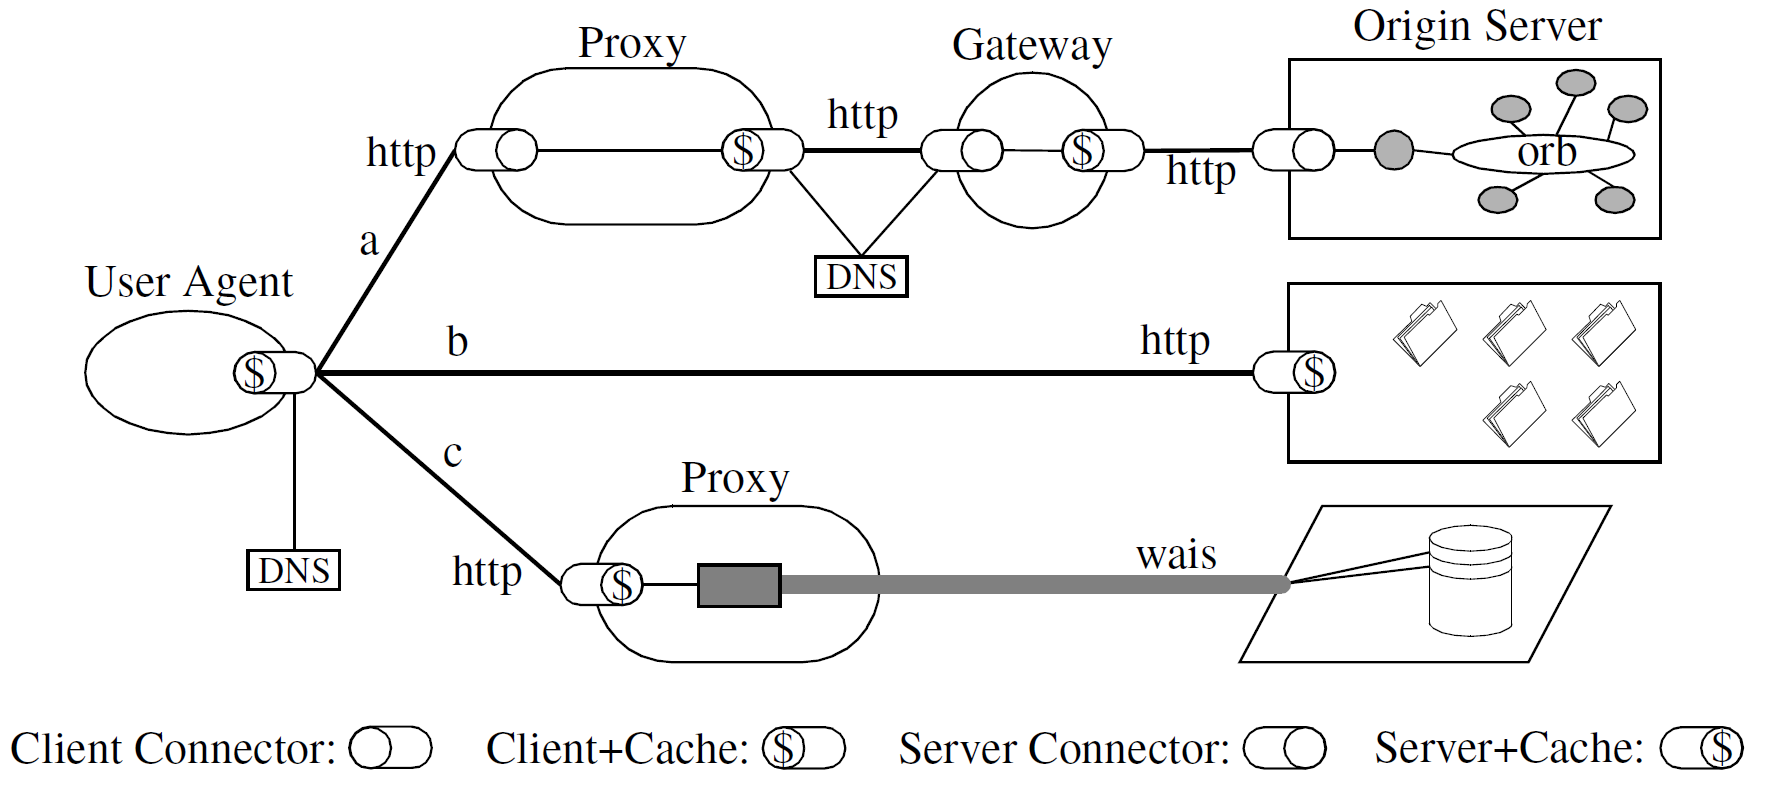
\includegraphics[width=\linewidth]{../Kapitel/Grafiken/REST-process-view.png}
  \caption{REST~\cite[84]{REST}}\label{img:REST-diss}
\end{figure}

\section{Implementierung von RESTful APIs}
Die REST Architektur ist generell protokollunabhängig, durch die Arbeit von Fielding an HTTP und URI sind diese jedoch sehr geeignet für die Implementierung und waren auch das erste Anwendungsfeld.\cite[vgl.][109,116]{REST}
Eine API, die dem REST Architekturstil folgt, wird RESTful genannt.
Da die Dissertation von Fielding jedoch einige Implementierungsdetails schuldig bleibt bzw.\ bewusst \textcquote[86]{REST}{Details der Komponentenimplementierung und Protokollsyntax [ignoriert]}, wurde der Begriff RESTful API mit der Zeit aufgeweicht und für APIs verwendet, die grundlegende Anforderungen nicht erfüllen.\cite[vgl.][]{fieldBlog}
\par
\begin{itemize}
  \item Richardson Maturity Model ermöglicht Bestimmung wie REST konform Web service (API) ist
  \item Level 0
  \item Level 1
  URI
  \item Level 2
  \begin{itemize}
    \item HTTP Methoden genutzt als Kontrolldaten um Intention auszudrücken
    \item CRUD Operationen werden abgedeckt
    \item GET:\ Anfragen einer Repräsentation der Ressource
    \item POST:\ kann zum Erstellen, Modifizieren und Löschen von Ressourcen verwendet werden, schlecht definiert; Funktionsweise in folgende Methoden aufgeteilt
    \item PUT:\ Erstellen/Ersetzen einer Repräsentation
    \item PATCH:\ Modifizieren einer Repräsentation
    \item DELETE:\ Löschen der Ressource
    \item GET, PUT, DELETE sind idempotent (gleiches Ergebnis bei mehrmaliger Ausführung). GET ist safe (kein Verändern der Ressource).
  \end{itemize}
  \item Level 3
  \begin{itemize}
    \item Hypermedia ermöglicht Navigation durch die API\@. Client ändert seinen Zustand, indem er URIs (Links) folgt (HATEOAS)
    \item keine externe Dokumentation nötig. Links zwischen Dokumenten dokumentieren die Ressourcen
    \item Datenformat ist entscheidend. Bestimmte Formate haben native Unterstützung für Links und Forms (HTML, ATOM)
    \item Media Type bestimmt Auswertung (und Anzeige) der Antwort. JSON, XML können genutzt werden. Client benötigt Informationen über Datenstruktur, um Links in diesen Dokumenten auszuwerten.
  \end{itemize}
\end{itemize}

\section{Verbreitung und Standardisierung}
\begin{itemize}
  \item REST bestimmt nicht welches Format benutzt werden muss.
  \item Kein REST Standard
  \item REST APIs nutzen Web Standards (HTTP, URI, Hypermedia)
  \item XML und HTML zur direkten Anzeige geeignet. JSON beliebter geworden, das leichter für Menschen und Maschinen zu lesen
  \item verschiedene Ansätze um Struktur von JSON Dokumenten zur Verwendung in APIs zu definieren. Teilweise miteinander verwendbar (definieren verschiedene Aspekte der Kommunikation)
  \item OpenAPI
  \item JSON:API
  \item Abbildung Beispiel Request und Response
\end{itemize}
REST bleibt Implementierungsdetails schuldig\cite[vgl.][86]{REST}
\chapter{GraphQL}

\section{Entwicklung und Grundgedanke}
\begin{itemize}
  \item GraphQL ist Abfragesprache für APIs und Laufzeitumgebung um auf Abfragen zu antworten
  \item Server stellt Schema = komplette Beschreibung der Datenstruktur
  \item Client sendet beliebige Abfrage und erhält exakt die angefragten Daten
  \item Eine Anfrage für alle nötigen Daten (für eine View, UI basiert); Vorteil bei langsamen mobilen Netzwerken
  \item 2012 von Facebook entwickelt und eingesetzt
  \item 2015 open source, GraphQL Foundation, Spec auf Github weiterentwickelt, Juni 2018 letzter Release
  \item Besteht aus Typsystem, Abfragesprache, Ausführungssemantik, statischer Validierung und Typintrospektion
\end{itemize}

\section{Spezifikation und Funktionsweise}
\begin{itemize}
  \item Typsystem
  \begin{itemize}
    \item Typsystem und GraphQL Schema drücken aus, welche Objekte die API zu Verfügung stellt
    \item Schema besteht aus `type', `enum' und `interface'. `type' kann `interface' implementieren
    \item jeder Type (und Interface) ist Ansammlung von Feldern
    \item `null' ist erlaubter Wert. Non-nullable Feld wird mit `!' markiert
    \item Einstiegspunkt (Top level) in Typsystem ist Objekttyp, Name nach Konvention `query'
    \item Felder auf query Typ sind mögliche Operationen; Argumente möglich
  \end{itemize}
  \item Query Syntax
  \begin{itemize}
    \item Abbildung Beispiel Query
    \item GraphQL Abfrage beschreibt deklarativ welche Daten erwartet werden
    \item Antwort ist JSON mit der gleichen Struktur
    \item Abfragen können geschachtelt werden
    \item Fragmente
    \begin{itemize}
      \item Abbildung Beispiel Fragment
      \item verhindert Dopplung von mehreren Feldern in Abfrage
      \item ermöglicht typbasierte Feldselektion
    \end{itemize}
  \end{itemize}
  \item Introspektion
  \begin{itemize}
    \item Spezialfelder beginnend mit doppelt Unterstrich
    \item \_\_schema, \_\_typename
    \item Metadaten über GraphQL Schemaß
    \item Sinn ist Nutzung durch Entwicklungstools
    \item ermöglicht statische Validierung: GraphQL Abfrage kann zu Entwicklungszeit geprüft werden
  \end{itemize}
  \item Referenzen werden unsichtbar, da von GraphQL Server automatisch aufgelöst (Performance beachten!)
  \item ein Endpunkt (kein Nutzen von URIs)
  \item jede Abfrage mit POST (kein Nutzen von HTTP Methoden)
  \item Semantik der Abfrage von Server ausgewertet (welche der CRUD Operationen)
\end{itemize}

\section{Server-Execution}

\chapter{Vergleich}
\section{Testumgebung}
Für den Vergleich der beiden API Ansätze wurde eine Single-Page Anwendung mit dem Vue.js Framework als Client und jeweils eine REST API und GraphQL API mit der Node.js Serverlaufzeitumgebung entwickelt.
Als Datenquelle dient zum einen eine MongoDB Datenbank, sowie Dateien im JSON Format.
Durch die Verteilung der jeweiligen Softwarekomponenten auf physikalisch unterschiedliche Rechner lassen sich mehrere Anwendungsfälle abbilden.
So wurden die Clientanwendung, die Serveranwendungen und die Datenbank in verschiedenen Kombinationen lokal und von Cloudumgebungen (Azure, Heroku, MongoDB Atlas) gehostet und ausgeführt.
Die JSON Dateien als Alternative zur Datenbank ermöglichen es, das Kontingent der Clouddatenbank nicht unnötig zu belasten und den durch Datenbankabfragen entstehenden Overhead, auf die deutlich schnellere Dateilesezeit zu minimieren.
Bei den Messungen wurde auf das Angleichen der Testbedingungen geachtet, besonders die im Zusammenhang mit Clouddiensten gemessenen Werte sind jedoch stark von der je nach Tageszeit unterschiedlichen, unbekannten Belastung des Dienstes abhängig.
\begin{figure}[h]
  \centering
  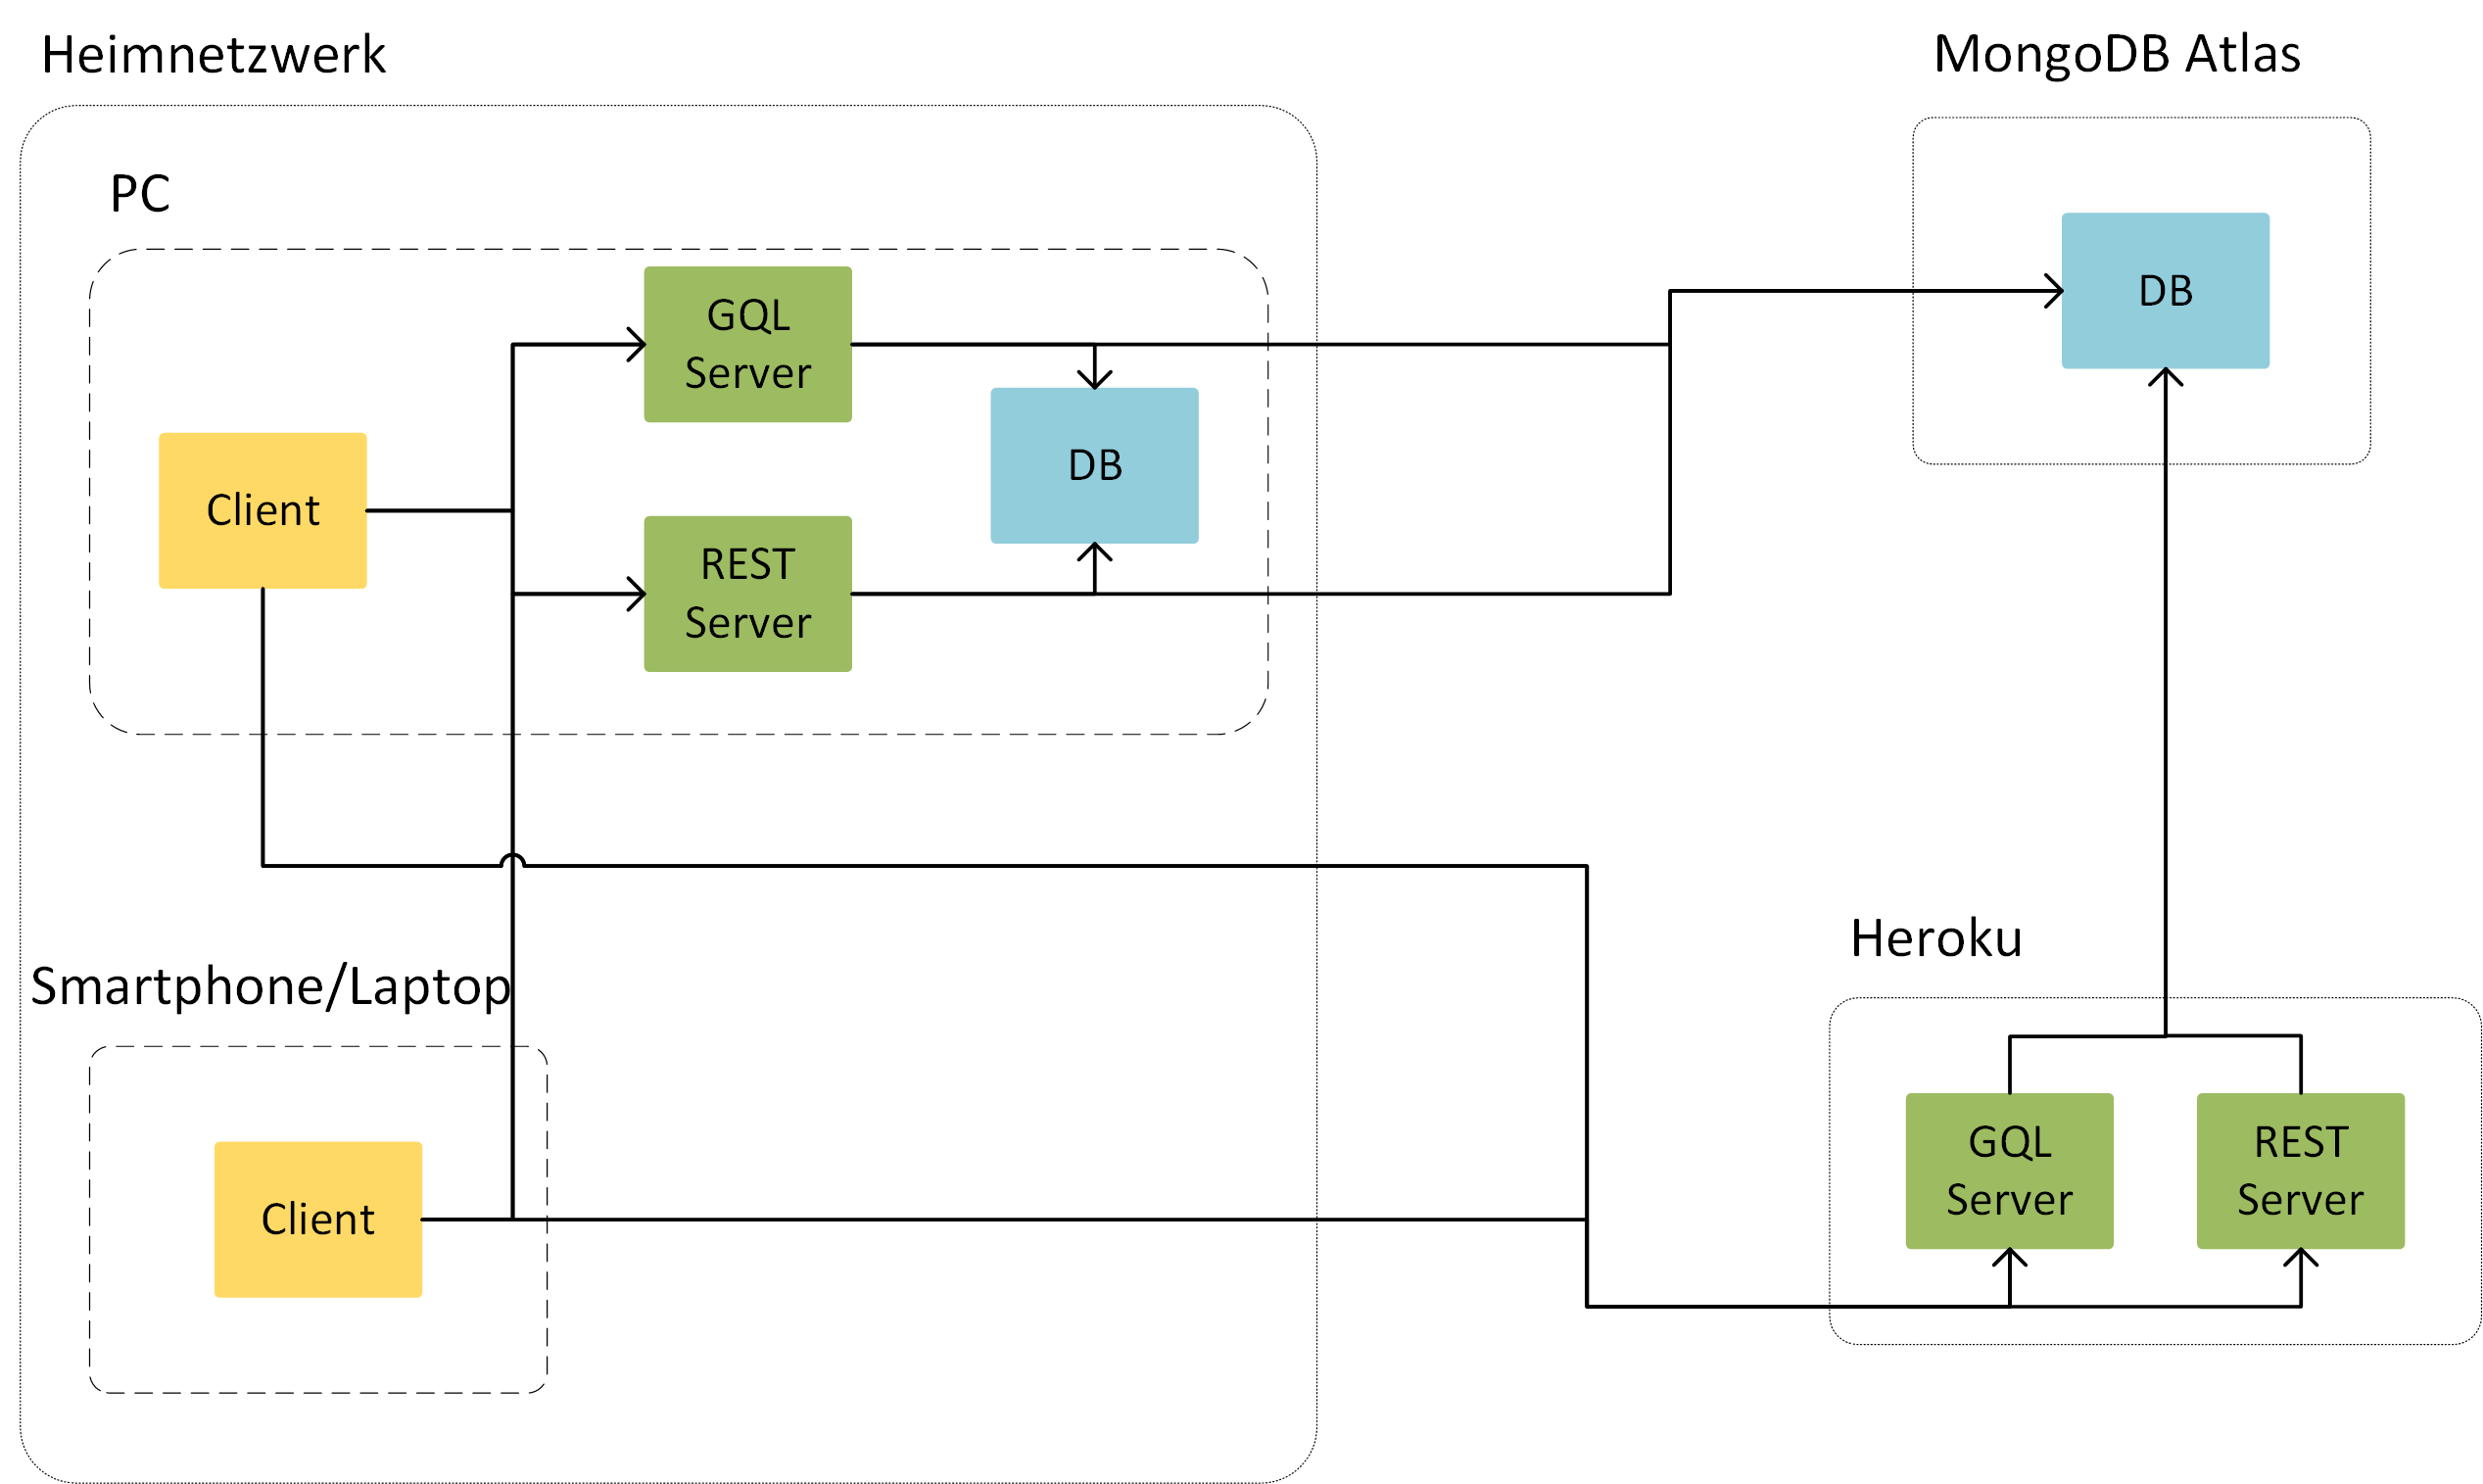
\includegraphics[width=\linewidth]{netzwerk.png}
  \caption{Architektur der Testumgebung}\label{img:netzwerk}
\end{figure}
\section{Abfrageflexibilität}
\begin{itemize}
  \item GraphQL
  \begin{itemize}
    \item unterscheidet Feldselektion, Sortieren, Filtern, Optionen
    \item keine Syntax für Sortieren/Filtern, aber Möglichkeit über Feldargumente
    \item an Query sind Performanceprobleme evtl.\ schwer erkennbar (siehe Tools)
  \end{itemize}
  \item REST
  \begin{itemize}
    \item fields=`` '' für Feldselektion
    \item field=`` '' zum Filtern
    \item sort=[field],sort-dir=desc zum Sortieren
    \item option=`` '' für Optionen
    \item includes empfohlen bei JSON:API, aufbrechen von HATEOAS\@?
  \end{itemize}
  \item Upload ist schwierig für GraphQL (serialization), REST kann multipart/form-data header nutzen
\end{itemize}
Bei der Entwicklung von Client-Anwendungen ist die Flexibilität der genutzten API ein entscheidender Einflussfaktor.
Dabei steht meistens die Flexibilität für das Generieren der Abfragen zum Empfangen von Daten im Vordergrund, aber auch Operationen zum Modifizieren von Ressourcen müssen betrachtet werden.
\par
GraphQL wurde als Abfragesprache entwickelt.
Eines der Entwicklungsziele ist es, dass eine Clientanwendung mit einer einzigen Abfrage alle für eine Ansicht nötigen Daten erhalten kann.
Der Server gewährt Zugriff auf das Datenschema, welches alle verfügbaren Daten und deren Relationen darstellt, sowie die Einstiegspunkte (Root Query), auf deren Basis ein Client seine Anfrage aufbauen kann.
Das Schema stellt den Rahmen für alle Abfragen dar.
Alle Daten, die der Server zur Verfügung stellt, werden durch Typen und deren Felder repräsentiert.
Jedes Feld, welches eine Clientanwendung erhalten möchte, muss in der Query angegeben werden.
Es existiert keine Möglichkeit, alle Felder eines Typs zu erhalten, ohne jedes davon anzugeben, \zB{} durch Wildcard Zeichen.
Der Client ist damit eng an das Schema gekoppelt, erhält aber auch nur die Daten, die tatsächlich angefragt wurden.
Die Möglichkeit eines GraphQL-Servers, beliebige Abfragen innerhalb des Schemas auszuwerten, eignet sich besonders für öffentliche APIs, bei denen dem API-Entwickler die individuellen Anforderungen und damit die Abfragen verschiedenster Anwendungen im Voraus nicht bekannt sind.
Die Relationen zwischen den Datentypen werden durch das Schema festgelegt.
Eine Anfrage kann jedoch beliebig viele, unabhängige Queries beinhalten, \zB{} um verschiedene Daten zu erhalten, die in keiner Beziehung zueinander stehen oder deren Beziehung durch das Schema nicht dargestellt wird.
Der Server kann für jedes Feld Parameter anbieten, welche die Auswertung des Feldwertes verändern.
Über solche Feldargumente können Optionen, die Geschäftslogik darstellen, aber auch allgemeine Abfragefunktionen, wie \zB{} Sortieren~\cite[vgl.][]{GraphQL-OrderBy} und Filtern~\cite[vgl.][]{GraphQL-Filter} zur Verfügung gestellt werden.
Einem Feld \enquote{Breite} könnte beispielsweise die Maßeinheit als Option übergeben werden.
\par
Während das Anfragen von Daten sehr viel Flexibilität für Clients bietet, ist das Modifizieren von Ressourcen nach Konvention nur über einzelne Mutations möglich.
Üblicherweise wird für jede Operation (Erstellen, Verändern und Löschen) einer Ressource eine separate Mutation zur Verfügung gestellt, welche durch den Namen eindeutig identifiziert wird.
Die Antwort auf eine Mutation kann wieder ein Objekt sein und genutzt werden, um das Resultat der Operation zu übermitteln oder den neuen Stand der Ressource abzufragen.
\par

In einer REST API ist jede Ressource über einen separaten Endpunkt erreichbar.
Das Veröffentlichen einer neuen Ressource geschieht durch das Einführen eines neuen Endpunktes.
Ein Endpunkt kann alle Methoden zum Abfragen und Ändern einer Ressource bereitstellen und durch die HTTP Verben semantisch unterscheiden.
Die Antwort auf einen GET Request an einen Endpunkt enthält alle Felder der Ressource bzw.\ die komplette Repräsentation.
In Beziehung stehende Daten, die nicht Teil einer Ressource sind, müssen über mehrere Requests vom Server angefragt werden.
Der Grundgedanke von HATEOAS ist, dass diese verbundenen Ressourcen Verweise aufeinander enthalten, wodurch ihre Beziehung dargestellt wird.
Das Zusammenbauen von Requests anhand der Links in erhaltenen Ressourcen ermöglicht große Flexibilität, erfordert jedoch, dass Daten erst ausgewertet werden müssen und danach erst neue Anfragen abgesetzt werden können.
Dadurch ist das Datenmodell nicht durch ein Schema vorgegeben, sondern kann zur Laufzeit geändert und explorativ genutzt werden, da es selbstdokumentierend ist.
Oftmals ist bei der Entwicklung von Clientanwendungen die erforderliche Datenstruktur jedoch bekannt und ist es wünschenswert, möglichst alle benötigten Informationen von wenigen Endpunkten zu erhalten, um die Performance zu steigern.
Dazu gibt es verschiedene Ansätze, wie der Query-String einer URI genutzt werden kann, um in Beziehung stehende Daten mit einem einzigen Request von einem Endpunkt zu erhalten.
Weder REST noch HTTP spezifizieren Syntax und Semantik des Query Strings bzw.\ betrachten diese als Implementierungsdetail.
Query-Parameter und Matrixparameter werden häufig gebraucht, um die Möglichkeiten von Abfragesprachen für REST zu implementieren.
Sie ermöglichen \zB{} die gewünschten Felder des angefragten Objektes, ein Feld nach dem sortiert oder ein Feld und Wert nach dem gefiltert werden soll, anzugeben.
Somit können Clientanwendungen die Antwort je nach ihren Anforderungen besser beeinflussen.
Abhängig davon wie unterschiedlich diese sind, muss die Entscheidung über die Erweiterung der Parameteroptionen oder das Einführen eines separaten Endpunktes getroffen werden.
Über sogenannte \enquote{includes} lassen sich bei JSON:API verbundene Objekte in die Antwort einbeziehen.
Includes sind außerdem eine effektive Lösung für das N+1 Problem.
Diese speziellen Auswertungen des Query-Strings müssen durch den REST Server angeboten werden und sind aus Entwurfssicht ein Tausch von erhöhter Abfragekomplexität und Clientflexibilität gegen Serverperformance.
\par
Da GraphQL für die Übertragung von Daten in Textform konzipiert wurde, müssen Informationen als Text vorliegen oder serialisiert werden.
Das kann besonders beim Hochladen von Binärdaten, wie Audio- oder Videodateien, zu sehr großen Datenmengen führen.
Eine REST API kann Binärdaten mit dem MediaType \enquote{multipart/form-data} empfangen und verarbeiten.
Für eine GraphQL API muss entweder ein Dateiupload-Service vorgeschaltet sein und nur der Link übertragen oder eine Bibliothek, wie \enquote{graphql-upload}, verwendet werden.

\section{Weiterentwicklung und Versionierung}
\begin{itemize}
  \item GraphQL
  \begin{itemize}
    \item neue Felder hinzufügen ohne existierende Queries zu beeinflussen
    \item neue Felder nicht automatisch gesendet
    \item Felder als deprecated markieren → Tool kann Entwickler warnen
    \item Monitoring auf Feldlevel möglich
  \end{itemize}
  \item REST
  \begin{itemize}
    \item Monitoring: werden sparse fieldsets oder includes verwendet können genutzte Felder aufgezeichnet werden
    \item neue Version, neuer Endpunkt example.com/v2/contacts/\dots
    \item für kleine Veränderungen ungeeignet
    \item Hinzufügen von Ressourcen → keine Versionierung notwendig
    \item Semantische Versionierung
    \item Hinzufügen/Umordnen von einzelnen Elementen sollte Client akzeptieren
    \item Versionierung über Accept-Header, URI oder query string
  \end{itemize}
\end{itemize}
\par 
Langlebige Software befindet sich in ständiger Entwicklung.
Ein Server muss auf Veränderungen des der API zugrunde liegenden Datenmodells reagieren können und diese gegebenenfalls Clients zugänglich machen.
Neue Anforderungen an die API erfordern das Erweitern der Abfragemöglichkeiten oder das Verringern derselben, wenn alte Funktionalität nicht mehr unterstützt oder durch neue ersetzt werden soll.
Da jede API einen Vertrag zwischen Server und Client darstellt, sollten Veränderungen einem festgelegten Ablauf und Kommunikationskanal folgen, um sukzessive Migration zu gewährleisten und Abfragefehler zu vermeiden.
Zu diesem Zweck wird in der Softwareentwicklung häufig Versionierung verwendet, bei der durch eine Zahl oder Zahlenkombination ein bestimmter Stand der Software bereitgestellt oder abgefragt wird.
\par
Um eine REST API um zusätzliche Ressourcen zu erweitern, ist keine Versionierung notwendig.
Stattdessen wird ein neuer Endpunkt hinzugefügt und über die Verlinkung von anderen Ressourcen oder als Einstiegspunkt in der Dokumentation bekanntgemacht.
Eine API Clientanwendung sollte so entwickelt werden, dass eine Antwort ausgewertet werden kann, solange sie semantisch eindeutig verständlich ist (Postel'sches Gesetz).
Das Umordnen und Hinzufügen von Elementen innerhalb einer Antwort sollte somit nicht zu Fehlern führen und die Validierung demgegenüber tolerant sein.
Normalerweise muss erst versioniert werden, wenn keine Rückwärtskompatibilität mehr gewährleistet werden kann.
Eine neue Version einer Ressource kann über mehrere Wege bereitgestellt und angefragt werden.
\begin{enumerate}
  \item Jeder Request kann einen Accept-Header enthalten, der zur Identifikation der zu sendenden Repräsentation genutzt werden kann.
  Sendet ein Client \zB{} einen Accept-Header mit dem Wert application/vnd.format.v2+json, so kann der Server durch Content-Negotiation anhand des \enquote{v2} die zu sendende Version ermitteln.
  \item Die URI als Identifikationsmittel kann ebenfalls genutzt werden, um verschiedene Versionen einer Ressource kenntlich zu machen.
  Die Anfrage an example.com/v2/events entspricht dem Erstellen eines neuen Endpunktes.
  Der Server muss nun auf einem weiteren Endpunkt antworten können, die Komplexität jedes einzelnen Endpunktes wird jedoch nicht erhöht.
  \item Für kleine Änderungen, wie das Ändern oder Entfernen eines einzelnen Feldes, ist normalerweise kein neuer Endpunkt nötig.
  Würde für jede dieser verhältnismäßig kleinen Änderungen ein neuer Endpunkt erstellt werden, ginge schnell die Übersichtlichkeit über die Menge der Endpunkte und deren Unterschiede verloren.
  Die URI der Ressource kann für verschiedene Versionen genutzt werden und stattdessen die Versionsinformationen im Query String transportiert werden (\zB{} example.com/events?version=2).
  Diese Variante teilt den gleichen Nachteil, den alle Query String Optionen haben, dass der Serverhandler für diesen Endpunkt komplexer und die Performance verringert wird.
  Es ist denkbar, dass nicht nur jede einzelne Option geprüft werden muss, sondern dass die Option für die Version der Ressource auch Auswirkung auf andere Optionen hat, sodass der Server einen Entscheidungsbaum auswerten muss, bevor eine Antwort gesendet werden kann.
\end{enumerate}
Wurde eine neue Version einer Ressource zur Verfügung gestellt, muss diese auch erreichbar sein.
Da die Änderungen von Variante 2 und 3 sich allein auf die URI auswirken, müssen in verknüpften Ressourcen die Links zur neuen Version aktualisiert werden.
Da Header in einem Link nicht repräsentiert werden können, ist es bei der ersten Variante notwendig, dass der Client über die neue Version informiert wird und allen Anfragen an die Ressource den Accept-Header hinzufügt.
\par
Beim Entfernen von Funktionalität ist es sinnvoll, die aktuelle Nutzung derselben durch Monitoring festzustellen und notwendig, die geplanten Änderungen zu kommunizieren.
Da normalerweise die gesamte Repräsentation einer Ressource als Antwort gesendet wird, kann nur die Nutzung des Endpunktes und nicht die tatsächliche Notwendigkeit einzelner Teile der Ressource bzw.\ Felder ermittelt werden.
Das ist jedoch möglich, wenn bei jeder Anfrage mittels Includes die gewünschten Felder angegeben werden müssen.
Sollen einzelne Elemente einer Ressource nicht mehr gesendet werden, so können diese zeitweise den für den Datentyp üblichen Nullwert enthalten, bevor sie endgültig entfernt werden.
Wird ein Endpunkt der API entfernt, so sollte der Server mit dem entsprechenden HTTP Status Code (410 Gone) antworten und alle Links in verknüpften Ressourcen müssen gelöscht werden.
Ist eine Ressource lediglich unter einem anderen Endpunkt erreichbar, so kann der Code 310 \enquote{Moved Permanently} den Client automatisch zur neuen URI weiterleiten.
\par
Erklärtes Ziel von GraphQL ist es, Versionierung zu verhindern und stattdessen die API kontinuierlich, abwärtskompatibel weiterzuentwickeln.
Da jedes Feld, welches ein Client erhalten möchte, in der Query explizit angegeben werden muss, ist detailreiches Monitoring bis auf Feldebene möglich.
Im Datenmodell neu eingeführte Felder beeinflussen bestehende Abfragen nicht, können aber jederzeit in diese aufgenommen werden.
Felder, die zukünftig aus der API entfernt werden sollen, können mit isDeprecated als veraltet gekennzeichnet und ein Grund als Metainformation angegeben werden.
Diese Kennzeichnung beeinflusst die Abfrage des Feldes nicht, kann aber per Introspektion zur Entwicklungszeit von Tools abgefragt und dem Entwickler als Warnung angezeigt werden.
Enthält eine Abfrage Felder, die im Schema nicht mehr enthalten sind, schlägt die Abfrage fehl.
Änderungen in der Auswertungslogik einzelner Felder können über optionale Feldargumente bereitgestellt werden.
Auch diese beeinflussen bestehende Abfragen ohne diese Argumente nicht.
Für Feldargumente und Input Typen existiert zur Zeit noch keine Möglichkeit, diese als veraltet zu kennzeichnen, ist aber für den nächsten Release der GraphQL Spezifikation geplant.
Ein GraphQL Server stellt ein Schema und damit alle darin enthaltenen Abfragen unter einer URI bereit.
Ergibt sich die Notwendigkeit, eine neue Version unter einer anderen URI zu veröffentlichen, so können Abfragen die Schemata nicht verbinden und werden vom Server nur im Kontext eines Schemas ausgewertet.
\section{Performance}
Zum Vergleich der Abfrageperformance von GraphQL und REST wurden jeweils nacheinander eine Reihe von Abfragen durchgeführt und gemessen, um die Charakteristik der Daten zu erforschen.
Die kostenfreie Laufzeitumgebung von Heroku (Dyno) unterliegt einem monatlichen Stundenlimit und wird nach 30 Minuten, in denen keine Anfragen gestellt werden, in den Schlafzustand versetzt.
Erhält eine schlafende Dyno eine Anfrage, so wird sie nach einer kurzen Verzögerung wieder aktiv. TODO Zitat Heroku
Diese anfängliche Verzögerungszeit ist nach der angegebenen 30 minütigen Pause, in geringerem Maße aber auch nach nur wenigen Sekunden Inaktivität zu beobachten.\ref{img:abfrage-zeitverlauf}
Diese anfänglichen Ausreißer sind unabhängig von der verwendeten API, wurden aber aufgrund der hohen Schwankungen in den weiteren Untersuchungen nicht einbezogen. 
\begin{figure}[h!]
  \centering
  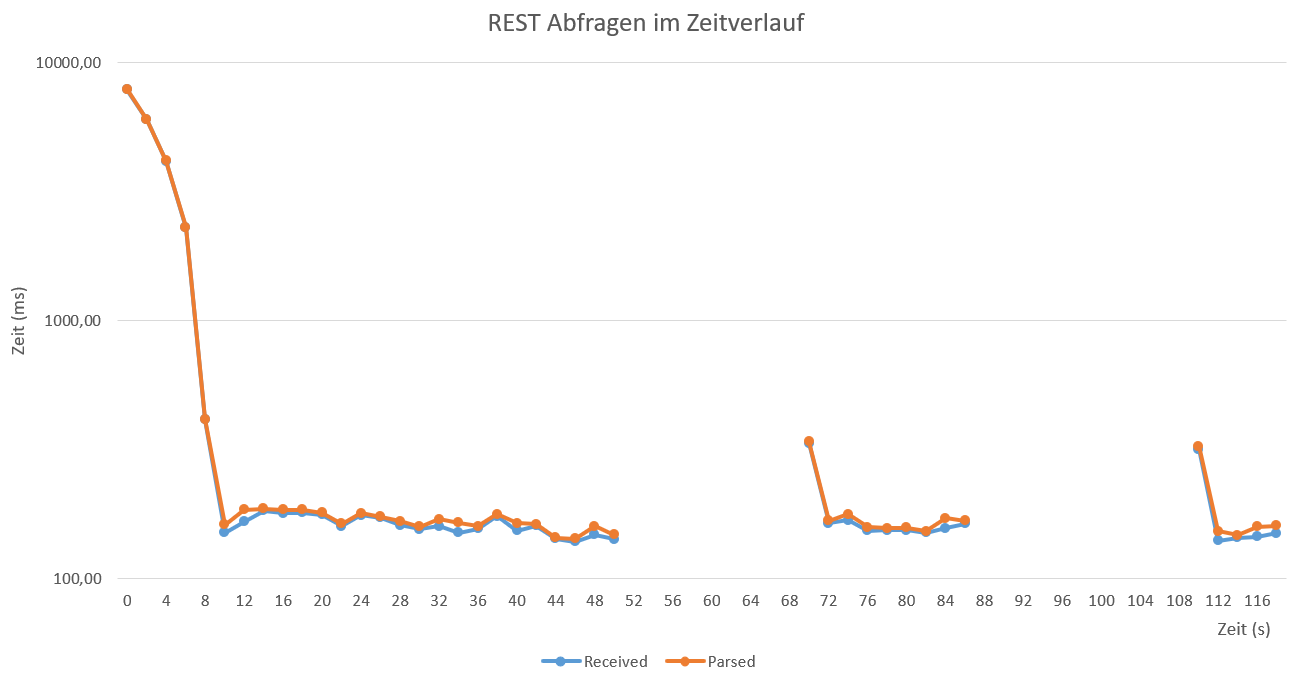
\includegraphics[width=\linewidth]{abfragen-zeitverlauf.png}
  \caption{Abfragen im Zeitverlauf}\label{img:abfrage-zeitverlauf}
\end{figure}
Je nach für die Abfrage verwendetem Gerät unterscheiden sich die Abfragezeiten deutlich.
\begin{figure}[h]
  \centering
  \begin{minted}{typescript}
    const startTime = performance.now();
    const response = await fetch('http://localhost:5000/events');
    const received = performance.now() - startTime;
    const data = await response.json();
    const parsed = performance.now() - startTime;
  \end{minted}
  \caption{Messung von Received- und Parsed-Zeit, Vereinfachte Darstellung aus \emph{EventFetch.vue} Z.~92f.}\label{code:measuring}
\end{figure}
\begin{figure}[h!]
  \centering
  \includegraphics[width=\linewidth]{abfrage-gerät2.png}
  \caption{Abfragen nach Gerät}\label{img:abfrage-gerät}
\end{figure}
\begin{figure}[h!]
  \centering
  \includegraphics[width=\linewidth]{parsing-gerät.png}
  \caption{Parsingzeiten nach Gerät}\label{img:parsing-gerät}
\end{figure}
\begin{figure}[h!]
  \centering
  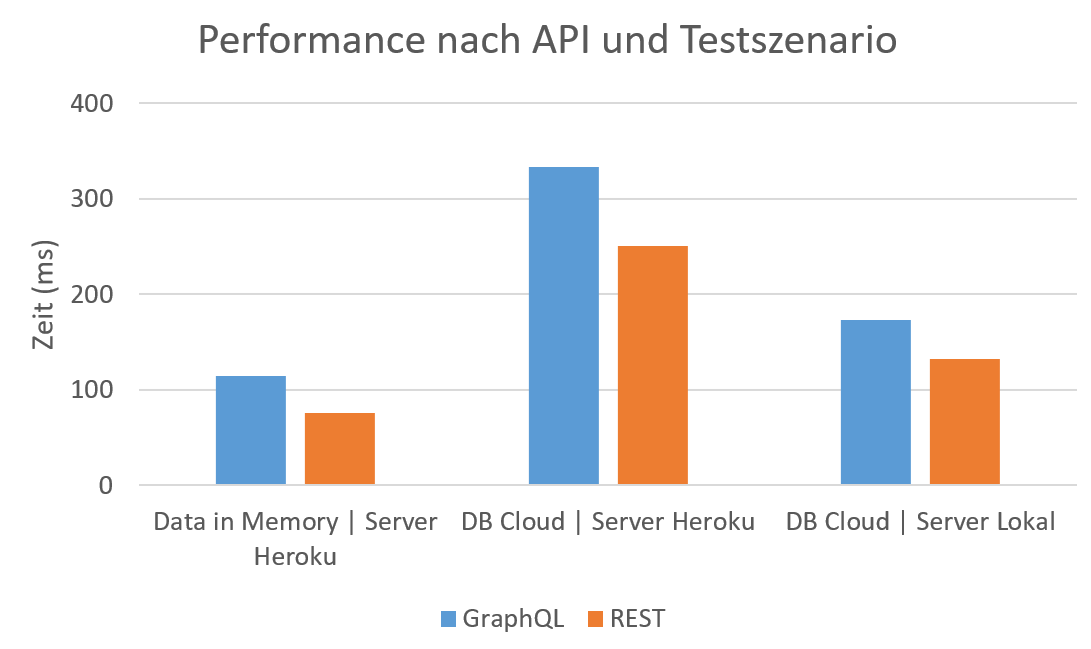
\includegraphics[width=\linewidth]{performance-szenario.png}
  \caption{Abfrageperformance nach Testszenario}\label{img:performance-szenario}
\end{figure}
\begin{figure}[h!]
  \centering
  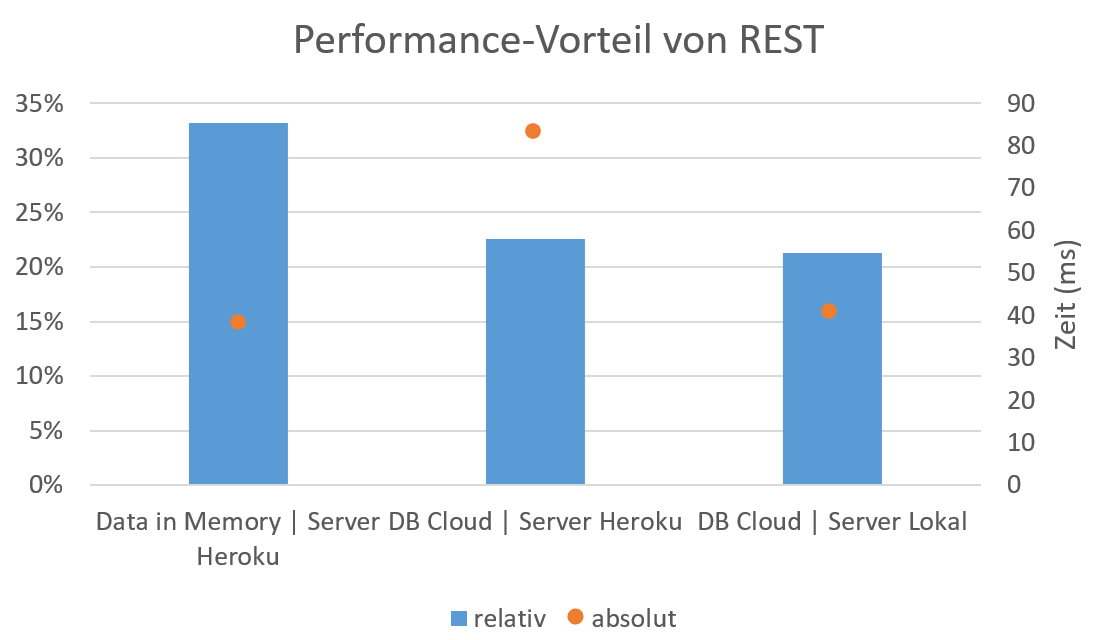
\includegraphics[width=\linewidth]{performance-diff.png}
  \caption{Performancedifferenz GraphQL-REST}\label{img:performance-diff}
\end{figure}

\section{Datenaufkommen/Netzwerklast}
\begin{itemize}
  \item Transfer, Verarbeiten und Speichern unnötiger Daten (Felder) sollte vermieden werden
  \item GraphQL
  \begin{itemize}
    \item automatisch kleinstmöglicher Request
    \item Query muss an Server gesendet werden
  \end{itemize}
  \item REST
  \begin{itemize}
    \item standardmäßig gesamte Repräsentation
    \item viele APIs bieten Feldselektion an (Partials)
    \item query string enthält Feldselektion nach bestimmter Syntax
    \item je komplexer, desto mehr Daten
    \item jede Ressource ist extra Endpunkt
    \item für mehrere Ressourcen müssen mehrere Requests gemacht werden, n+1 Problem
    \item includes beziehen verbundene Daten in Response ein → ein Request für mehrere Ressourcen
  \end{itemize}
  \item GraphQL und REST Partials unterscheiden Objekt und Array nicht → Wissen über API notwendig um Performance einzuschätzen
  \item mehr Daten um Request genauer zu machen, sinnvoll um deutlich weniger Daten als Response zu erhalten
\end{itemize}

\section{Caching}
\begin{itemize}
  \item Flexibilität gegen Caching: je spezieller die Abfrage, desto schwieriger (weniger sinnvoll) caching
  \item nicht Antwort direkt cachen (HTTP), sondern manuell Objekte anhand ID cachen (JavaScript)
  \item REST
  \begin{itemize}
    \item Browser HTTP caching automatisch genutzt
    \item Caching basierend auf Endpunkt
    \item URL ist cache ID für die Ressource
    \item ermöglicht HTTP cache proxies
    \item je spezieller der query string, desto weniger cache Treffer
  \end{itemize}
  \item GraphQL
  \begin{itemize}
    \item POST response wird normalerweise nicht gecacht
    \item standardmäßig keine ID für caching vorhanden. Empfehlung: API sollte ID pro Objekt bereitstellen
  \end{itemize}
\end{itemize}

\section{Batching/Deduping}
\begin{itemize}
  \item GraphQL queries können parallel ausgewertet werden, Mutations nicht
\end{itemize}

\section{Fehlerbehandlung}

\section{Sicherheit}

\section{Kosten}

\section{Lernkurve, Fehlersuche, Community}

\section{Bibliotheken und Tools}
\begin{itemize}
  \item GraphQL
  \begin{itemize}
    \item offizielle Spezifikation vorhanden
    \item Referenzimplementierung in JavaScript
    \item Zusatztools von Facebook (Dataloader, Relay)
    \item Tool kann Abfragekomplexität zu Entwicklungszeit ermitteln (mit vergangenen Messwerten)
  \end{itemize}
  \item REST: fehlende Standards (in Bezug auf linkelemente) macht die Entwicklung von Tools schwierig
\end{itemize}

\section{Fazit und Auswertung}

\subsection{Zusammenfassung}

\subsection{Kombinierte Verwendung von GraphQL und REST}

\subsection{Ausblick}

\input{../Kapitel/kapitel7.tex}

\printbibliography[title=Literaturverzeichnis]

\addchap{Anlagen}
\input{../Selbständigkeitserklärung/selbständigkeitserklärung.tex}

\afterpage{\blankpage}

\end{document}